\documentclass[tikz]{standalone}


\usepackage{forest,xcolor}
\usetikzlibrary{matrix, positioning}

\begin{document}
  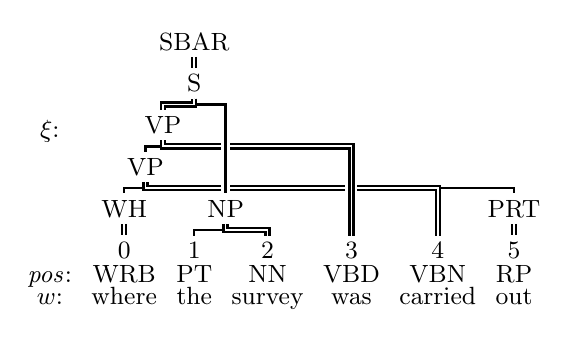
\begin{tikzpicture}[
      edge from parent path={(\tikzparentnode.south) -- ++(0,-.5ex) -| (\tikzchildnode.north)},
      every path/.style={line width=.2ex},
      level distance=3.5ex,
%      node distance=3ex,
      anchor=center,
      every node/.style={font=\small}
    ]
    \matrix (pos) [matrix of nodes, outer sep=0pt, inner sep=0pt, row sep=0pt, column sep=7pt] {
      \(\mathit{pos}\): & WRB   & PT  & NN      & VBD & VBN     & RP  \\
      \(w\):            & where & the & survey  & was & carried & out \\};
    \node[above=10ex of pos-1-1] {\(\xi\):};

    \tikzstyle{headnode} = [] % [draw=lightgray, dashed]

    \begin{scope}[every node/.style={inner sep=2pt, font=\small}]
        \node[above=17.5ex of pos-1-3] (sbar) {SBAR}
        child { node[headnode] (s) {S}
            child { node[xshift=1em, headnode] (vp1) {VP}
                child { node[xshift=1.5em] (vp2) {VP}
                    child { node[above=3.5ex of pos-1-2] (wh) {WH} child {
                            node (term0) {0}
                            edge from parent[double]}}
                    child {
                        node[above=0ex of pos-1-6, headnode] (term4) {4}
                        edge from parent[double]}
                    child { node[above=3.5ex of pos-1-7] (prt) {PRT} child {
                            node (term5) {5}
                            edge from parent[double]}}}
                child {
                    node[above=0ex of pos-1-5, headnode] (term3) {3}
                    edge from parent[double] }
                edge from parent[double]}
            child { node[xshift=-1em,yshift=-7ex] (np) {NP}
                child { node[above=0ex of pos-1-3] {1} }
                child {
                    node[above=0ex of pos-1-4, headnode] (term2) {2}
                    edge from parent[double] }}
            edge from parent[double]};
    \end{scope}

      % redraw corssing edges with white foundation
      \begin{scope}
      	%%%%%%%%%%%%%%%%%%%%%%%%%%%%%%%
      	% redraw edge to term4, to avoid filling its gap by the edge to term5
      	\draw[double] (vp2.south) -- ++(0,-.5ex) -| (term4.north);
      	%%%%%%%%%%%%%%%%%%%%%%%%%%%%%%

        \draw[white, line width=1ex] (vp1.south) -- ++(0,-.5ex) -| (term3.north);
        \draw (vp1.south) -- ++(0,-.5ex) -| (vp2.north);
        \draw[double] (vp1.south) -- ++(0,-.5ex) -| (term3.north);

        \draw[white, line width=.7ex] (s.south) ++(.5pt,-.5ex) -| (np.north);
        \draw (s.south) -- ++(0,-.5ex) -| (np.north);
        \draw[double] (s.south) -- ++(0,-.5ex) -| (vp1.north);
      \end{scope}

  \end{tikzpicture}
\end{document}
